\section{Design af spoler}\label{sec:sec_spole_design}

\subsection{Dimensionering af spoler}

Systemet består af 3 spoler. 1 stor spole til at vidergive et signal, og 2 mindre spoler med samme areal til at opfange et signal. Dimensioneringen afhænger af størrelserne på spolerne. Der er nogle fysiske pladskrav, som begrænser dimensioneringen. Som udgangspunkt, dimensioneres den store spole først, som skal sende et signal videre. (omformuler blot udkast..)

Figur her!!

\begin{figure}[h!]
	\centering
	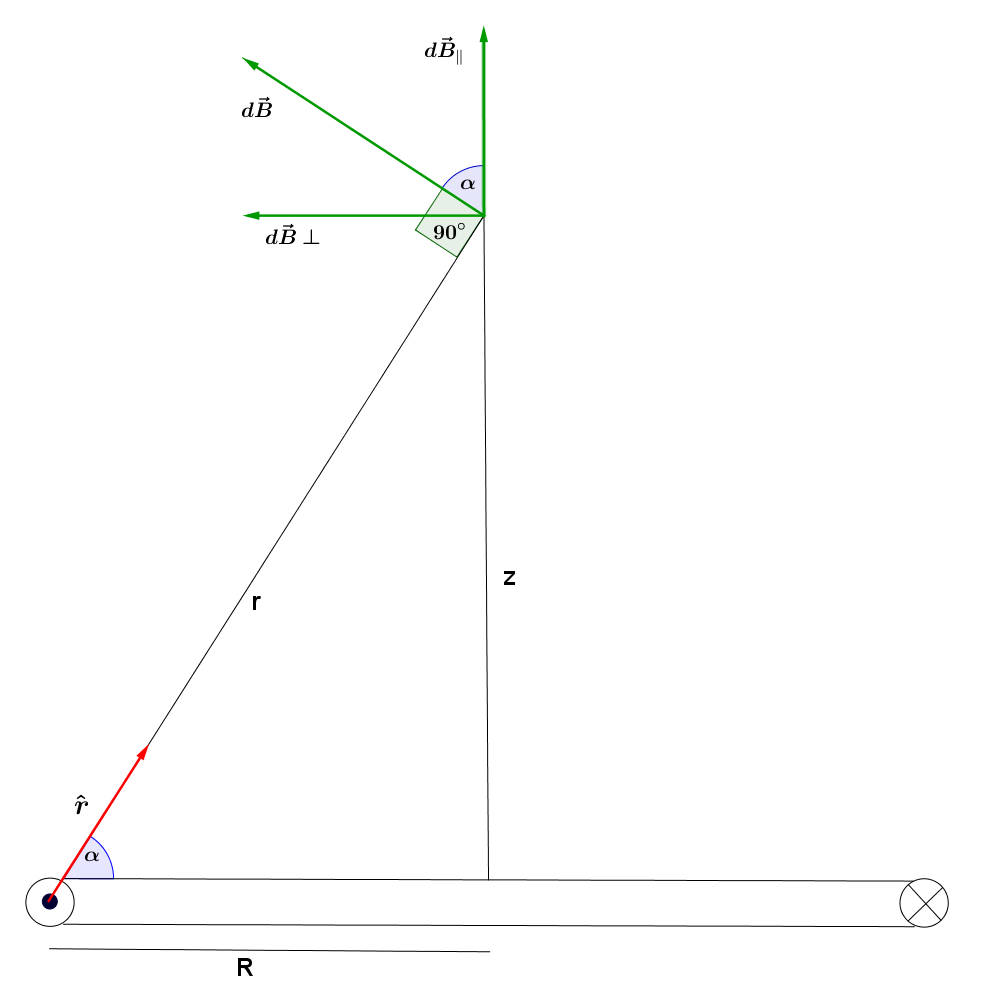
\includegraphics[width=.6\textwidth]{billeder/B_felt.png}
	\caption{test}
	\label{fig:BiotSavart1}
\end{figure}

 \begin{align}
 	&\vec{r'}=R(cos(\phi)\hat{i}+sin(\phi)\hat{j})
 \end{align}

\begin{align}
	&id\vec{s}=i\frac{d\vec{r'}}{d\phi}=i R d\phi (-sin(\phi)\hat{i}+cos(\phi)\hat{j})
\end{align}
Stedvektor:
\begin{align}
	&\vec{r_p}=z\hat{k}
\end{align}

relativ stedvektor
\begin{align}
	&\vec{r}=\vec{r_p}-\vec{r'}=-R cos(\phi)\hat{i}-sin(\phi)\hat{j}+z\hat{k}
\end{align}

Biot-savarts lov:
\begin{align}
	&d\vec{B}=\frac{\mu_0  i}{4\pi} \frac{d\vec{s} \times \hat{r}}{r^2}
\end{align}

\begin{align}
	&\hat{r}=\frac{\vec{r}}{r}
\end{align}

\begin{align}
	&r= \mid \vec{r} \mid = \sqrt{R^2+z^2}=\mid \vec{r_p}-\vec{r'} \mid
\end{align}



ganger igennem med ovenstående. (ligning?)

\begin{align}
	&d\vec{B}=\frac{\mu_0 i}{4\pi} \frac{d\vec{s} \times \vec{r}}{r^3}
\end{align}

	
\begin{align}
	&d\vec{s}\times(\vec{r_p}-\vec{r'})=R d\phi (-sin(\phi)\hat{i}+cos(\phi)\hat{j})\times (-R cos(\phi)\hat{i}-sin(\phi)\hat{j}+z\hat{k})
\end{align}	
Som yderligere kan reduceres ned til:

\begin{align}
	R \phi (z cos(\phi)\hat{i}+z sin(\phi)\hat{j}+R\hat{k})
\end{align}

\begin{align}
	&d\vec{B}=\frac{\mu_0 i}{4\pi} \frac{d\vec{s}\times (\vec{r_p}-\vec{r'})}{(\sqrt{R^2+z^2})^2}=\frac{\mu_0 i}{4\pi} \frac{R \phi (z cos(\phi)\hat{i}+z sin(\phi)\hat{j}+R\hat{k})}{(R^2+z^2)^\frac{3}{2}}
\end{align}


Ud fra dette, kan x og y komposanterne af B feltet sættes til = 0. Dette bevises ud fra:
\begin{align}
	&\frac{\mu_0 R z}{4\pi} \int\limits_{0}^{2\pi}cos(\phi)d\phi = 0
\end{align}


\begin{align}
	&\frac{\mu_0 R z}{4\pi} \int\limits_{0}^{2\pi}sin(\phi)d\phi = 0
\end{align}

Herefter er der kun z komposanten tilbage:
\begin{align}
	&B=\frac{\mu_0 R z}{4\pi} \int\limits_{0}^{2\pi}d\phi
\end{align}

Og dermed et udtryk for B i en cirkel.... (ret tekst her samt alle andre steder ved udledning.):


\begin{align}
	&B=\frac{\mu_0 iR^2 2\pi}{2(R^2+z^2)^\frac{3}{2}}
\end{align}




Tekst omkring solenoid her samt figur.



\begin{align}
	&di=inz'
\end{align}

\begin{align}
	&n=\frac{N}{L}
\end{align}

\begin{align}
	&d\vec{B}=\frac{\mu_0 R^2}{2[(z-z')^2+R^2]^\frac{3}{2}}di = \frac{\mu_0 R^2 i n dz'}{2[(z-z')^2+R^2]^\frac{3}{2}}
\end{align}


B felt i et givet punkt P centreret ud fra z aksen, med funktion af z er dermed givet ved:
\begin{align}
	&B(z)=\frac{\mu_0 n R^2 i}{2}\int\limits_{0}^{2\pi}\frac{1}{2[(z-z')^2+R^2]^\frac{3}{2}}dz'
\end{align}

\begin{align}
	&B(z)=\frac{\mu_0 n i}{2}\bigg[\frac{\frac{L}{2}-z}{\sqrt{(\frac{z-L}{2})^2+R^2}}+\frac{\frac{L}{2}+z}{\sqrt{(\frac{z+L}{2})^2+R^2}}\bigg]
\end{align}

\subsection{3D design/fysisk design af spolehus}
\begin{itemize}
	\item Inventor
	\item PnP system
	\item Huller til vindingsmaskine
	\item Clamp
\end{itemize}
Spolerne er designet således at når den store spole er i nul (i midten) overlapper den de mindre spoler så de er dækket præcist 50\percent. Når den store spole så er i sin fulde udslagsvinkel er hhv. den ene mindre spole dækket helt, hvor den anden slet ikke er dækket. \\

Illustration af forklaring her...

\emph{Introduktion til emnet i kapitlet skrives her}
\begin {itemize}
\item Udnytter forudborede huller
\item Batteri"slots"
\item Standoff mounts til print

\item Udgangssignalet på spolen skal filtreres og ensrettes
\item Aktivt båndpas filter, fordele vs. passivt
\item Indsnævring af frekvens
\item Ensretteren/konvertering til DC
\item Regulator-venligt signal. 

\item 555 generator
\item Firkantsignal
\item Opsætning 
\item Modstandsbestemmelse
\end {itemize}

\section{Elektriske kredsløb}\label{sec:sec_sparningsreg}
Der vil i dette afsnit blive gennemgået alle de elektriske kredsløb der er anvendt til projektet. Til hvert kredsløb er der beskrevet problemstilling, hvordan det løses, hvordan beregningerne gennemgås for hvert enkelt komponent, samt hvordan det hele fungerer.
På pendulet sidder én stor spole parallelt overfor to mindre spoler. Der skal her sendes et signal ind på den store spole således at der opbygges at magnetfelt der overføres til de to mindre spoler via gensidig induktans. Til forsygning på bilen anvendes to batterier der symboliserer to DC kilder. Da der ikke kan opstå gensidig induktans i spoler ved DC skal der findes en alternativ løsning til at opnå et varrierende signal. Af brugbare signaler findes der firkant, trekant og sinus signaler.
...
\subsection{Systemforsyning}
\begin{itemize}
	\item +- 7V (?) til sensorer samt signalbehandling
	\item 2 batterier på 7.4V hver. 
	\item LiPo celler for mest afladekapacitet pga. motor som trækker en del
	\item Billige og tilgængelige
	
\subsection{Spændingsregulator}
\begin{itemize}
	\item Konstant x antal volt til frekvensgeneratoren
	\item Tager højde for voltage sag i LiPo batterier
\end{itemize}

	
	\subsubsection{Design}
	...
	
	\subsubsection{Beregninger}
	
	\begin{equation}
	\label{eq:RegulatorDesign}
	\begin{split}
	V_{in} & = 8.4V \\
	V_{out} & = 7V \\
	I_{in} & = 20mA \\
	I_Z & = 5mA \\
	I_{out} & = I_{in} - I_Z \\
	I_{out} & = 15mA \\
	R_1 & = \frac{V_{in} - V_{out}}{I_Z + I_{out}} \\
	R_1 & = 70 \Omega 
	\end{split}
	\end{equation}
	
	R1 er lig R2
	
	\begin{equation}
	\label{eq:RegulatorDesignTilnaermelse}
	\begin{split}
	R_1 & = 68 \Omega \\
	V_{out} & = V_{in} - I_{out} \cdot R_s - I_z \cdot R_s \\
	V_{out} & = 7.04V
	\end{split}
	\end{equation}
	
	\subsubsection{Virkemåde}
\end{itemize}


...

\subsection{Frekvensgenerator}

\subsubsection{Design}
Til at genererer et signal ud fra batterierne anvendes en timer kreds. Timeren skal her bruges til at lave et puls signal der har en given frekvens og duty cycle, dvs. et firkantet signal. Der er her valgt en konfiguration der hedder A-stabel. Fordelen ved dette er at timeren kan hente sit input direkte fra forsygning der i dette tilfælde er et batteri, dette koster en ekstra modstand men med den fordel at duty cycle og frekvens bliver frie variabler. Dette signal skal have en frekvens der er tilpas høj så systemet er mindre modtagelig overfor forstyrrelse og det vil give en hurtigere respons. Den astable konfiguration ser ud som på figur...\\

Der er dog den begrænsning at timeren kun kan lave et firkantet output. Hvis firkant signalet skal laves om til et sinus så kræver det nogle ekstra komponenter, hvilket betyder et potentielt langsommere system plus ekstra effekt afsættelse, og dermed en mindre spænding. For spolen betyder det ikke så meget om signalet er firkantet eller sinus formet, så længe det er et tidsvarierende signal, så opstår der gensidig induktans.\\

Den næste ulempe ved timeren er at den ikke kan lave en negativ spænding på udgangen. Det vil sige at signalet vil svinge mellem 0 og forsygningsspændingen. Dette er et problem fordi spolen ikke laver et varierende magnetfelt der varierer mellem plus og minus. For at løse dette problem skal der sættes en kondensator på udgangen. Denne kondensator skal regnes så dens impedans er meget mindre en spolens impedans ved den ønskede frekvens. Dette medfører at signalet på udgangen komme til at svinge mellem en positiv og negativ værdi, svarende til det halve af forsygningen.\\

Inden kredsløbet tegnes færdigt skal der tages højde for den spænding timeren leverer. Spolen har en meget lille indre modstand, hvilket medfører at ved høje spændinger, skal timeren leverer en stor strøm. Da timeren ikke kan holde til at leverer mere end $225 mA$, sættes en modstand i serie for at begrænse strømmen. Det færdige kredsløb ses på figur...

\subsubsection{Beregninger}
Til udregning af modstand og kondensatorværdier anvendes to af de ligninger der er opgivet i databladet for NE555 timeren. Først anvendes ligning 5 i data bladet til at bestemme modstanden $R_5$. Da der ikke er ligninger nok så bliver duty cyclen og modstanden $R_6$ valgt. Duty cyclen sættes til $51 \% $ , og $R_6$ vælges til $15k \Omega $. Ligning 5 i databladet omskrives svarende til i ligning \ref{eq:InputOmskrevet} .

\begin{equation}
\label{eq:InputOmskrevet}
R_5 = \frac{R_6}{D} - 2 \cdot R_6
\end{equation}

Parametrene indæsttes i ligning \ref{eq:InputOmskrevet}.
Resultatet viser her at $R_5$ skal være $588 \Omega $ for at opnå en duty cycle på $51 \% $.
\subsection{Forsyning og spændingsregulator}
\begin{equation}
\label{eq:InputsModstand}
\begin{split}
D & = 0.51\\
R_6 & = 15k \Omega \\
R_5 & = \frac{R_6}{D} - 2 \cdot R_6 \\
R_5 & = 588 \Omega 
\end{split}
\end{equation}

... 

\begin{equation}
\label{eq:TriggerKondensator}
\begin{split}
F_c & = 50kHz \\
C_7 & = \frac{1}{f \cdot \left( \frac{25 \cdot R_5 }{36} + \frac{25 \cdot R_6}{18} \right) }\\
C_7 & = 0.9nF
\end{split}
\end{equation}

...
\begin{equation}
\label{eq:TimerTilnaermedeVaerdier}
\begin{split}
R_5 & = 680 \Omega \\
C_7 & = 1nF \\
D & = 0.49 \\
F_c & = 46936Hz
\end{split}
\end{equation}

\subsubsection{Virkemåde}

...

\subsection{Båndpassfilter}
...

\subsubsection{Design}
...

\subsubsection{Beregninger}

\begin{equation}
\label{eq:FilterParametre}
\begin{split}
C_{filter} & = 470pF\\
H_o & = 3\\
Q & = 3\\
F_c & = 46936Hz \\
\omega_c & = 2 \cdot \pi \cdot F_c
\end{split}
\end{equation}

C10=C11=C17=C16

\begin{equation}
\label{eq:FilterModstandeBW}
\begin{split}
B & = \frac{F_c}{Q} \\
R_8 & = \frac{Q}{\omega_n \cdot C_{filter} \cdot H_o } \\
R_9 & = \frac{Q}{ \omega_n \cdot C_{filter} \cdot \left( 2 \cdot Q^2 - H_o \right) } \\
R_{10} & = \frac{2 \cdot Q}{ \omega_n \cdot C} \\
B & = 15645Hz \\
R_8 & = 7215 \Omega \\
R_9 & = 1430 \Omega \\
R_{10} & = 43288 \Omega
\end{split}
\end{equation}

R8 er lig R13. R9 er lig R14. R10 er lig R15.

\begin{equation}
\label{eq:FilterModstandeTilnaermelse}
\begin{split}
R_8 & = 6.8k \Omega \\
R_9 & = 1.5k \Omega \\
R_{10} & = 47k \Omega
\end{split}
\end{equation}

...

\begin{equation}
\label{FilterAendringer}
\begin{split}
F_c & = \frac{1}{2 \cdot \pi \cdot C} \cdot \sqrt{\frac{R_8+R_9}{R_8 \cdot R_9 \cdot R_{10}}} \\
H_o & = \frac{1}{\left( \frac{R_1}{R_3} \right) \cdot 2} \\
B & = \frac{F_c}{Q} \\
F_c & = 44557Hz \\
H_o & = 3.5 \\
B & = 14.9kHz
\end{split}
\end{equation}

\subsubsection{Virkemåde}
...

\subsection{Ensretter}

\subsubsection{Design}
...
\subsubsection{Beregninger}

\begin{equation}
\label{eq:EnsretterKondensator}
\begin{split}
V & = 2V \\
V_{rip} & = 300mV \\
R_{11} & = 5k \Omega \\
t & = 21 \mu S \\
i & = \frac{V}{R_{11}} \\
i & = 400 \mu A \\
C_{14} & = \frac{i \cdot t}{V_{rip} }\\
C_{14} & = 28nF \\
\tau & = R_{11} \cdot C_{14} \\
\tau & = 141 \mu S
\end{split}
\end{equation}

C14=C20. R11=R16

\begin{equation}
\label{eq:EnsretterKondensatorTilnaermelse}
\begin{split}
C_{14} & = 22nF \\
R_{11} & = 4.7k \Omega \\
\tau & = 103 \mu S
\end{split}
\end{equation}

\subsubsection{Virkemåde}

\subsection{Instrumenteringsforstærker}

\subsubsection{Design}
...

\subsubsection{Beregninger}

Indsæt billede af forstærker tabeller

\subsubsection{Virkemåde}
... 

\subsection{Regulator}
...

\subsubsection{Design}

....

\subsubsection{Beregninger}

...

\subsubsection{Virkemåde}

...
\section{Motorstyring}\label{sec:sec_motorstyring}

\begin{itemize}
	\item Omsætter volt til ampere (current control)
	\item Pnp og npn transistorer med relativ høj strømrate
	\item Motor accelererer baseret på ampere. Volt angiver tophastighed.
	\item Min 1.25A maks 2.25A
\end{itemize}

\subsubsection{Design}
...

\subsubsection{Beregninger}
..

\subsubsection{Virkemåde}
...